\question
Одним теплым вечером кот Степан вдохновился картинами, которые он увидел в Эрмитаже, и решил нарисовать свой автопортрет. Так как у Степана была тетрадка в клетку, оставшаяся после пройденного курса дискретной математики, он решил рисовать там. Нарисовав автопортрет ровно по клеткам, он подумал, что можно дорисовать координатные оси и обозначить все целые точки, пересекающиеся с контуром портрета. На обратной стороне листка он увидел конспект лекции по бинарным отношениям. Но так как память у кота не очень хорошая, он решил попросить вас найти бинарное отношение, соответствующее рисунку и два таких бинарных отношения, чтобы в композиции они давали исходное бинарное отношение и изобразить их.
\\
\begin{figure}[h]

\begin{minipage}[h]{0.55\linewidth}
\end{minipage}
\begin{minipage}[h]{0.45\linewidth}
\center{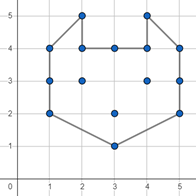
\includegraphics[width=0.7\textwidth]{pic/721.png} }
\end{minipage}
\end{figure}



---------------

Автор -- Алёна Холмогорова, М3209